%!TEX root = main.tex
%
%\newpage
%\appendix

\section{Derivation of the influence formula}
\label{si-sec:infl-derivation}

In this section, we detail the calculation of the tweet influence $\varphi(v)$, proposed by~\citet{Rizoiu2018a}.
%We start from an observed retweet cascade, for which the Twitter API does not provide the actual structure of the social network.
In Sec.~\ref{subsec:diffusion-scenario}, we define the notion of diffusion scenario, and we compute its likelihood given an observed retweet cascade.
In Sec.~\ref{subsec:user-influence}, we compute the formula for tweet influence over all possible diffusion scenarios associated with the given cascade.

\subsection{Diffusion scenarios}
\label{subsec:diffusion-scenario}

\textbf{Diffusion trees.}
We can represent an online diffusion using a directed tree $G(V, E)$, in which each node has a single parent and the direction of the edges indicates the flow of the information.
For retweet cascades, the nodes $v \in V$ are individual tweets and each directed edge $e \in E, e = (v_a, v_b)$ (showing the direction $v_a \longrightarrow v_b$) indicates that $v_b$ is a \emph{direct retweet} of $v_a$.
A direct retweet means that $u_b$ -- the user that emitted the tweet $v_b$ -- clicked on the ``Retweet'' option under tweet $v_a$.
The top panel of Fig.~\ref{fig:example-diffusion-graph-construction} shows an example of such a diffusion tree.
Note that each node $v$ has associated a time of arrival $t_v$ and that the diffusion tree respects the order of the times of arrival -- i.e. given the edge $e = (v_a, v_b)$, then $t_a < t_b$.
The bottom panel of Fig.~\ref{fig:example-diffusion-graph-construction} shows the incremental construction of the diffusion tree shown in top panel:
node $v_1$ is the root of the tree and the source of the information diffusion; 
at each time $t_i$, node $v_i$ attaches to the previous tree constructed at time $t_{i-1}$.

%We start from the graph representation of a social network, in which nodes correspond to users and the directed edges correspond to social ties -- following the updates of another user on Facebook, the following relation on Twitter etc.
%We can represent the diffusion of information in a social graph as a directed tree (as shown in Fig.~\ref{fig:example-diffusion-graph}).
%Fig.~\ref{fig:diffusion-graph-construction} shows the associated diffusion process:
%leaves attach to the tree sequentially, as the information propagation progresses.
%%the propagation process continues by sequentially attaching new leaves to this tree over time as shown in Fig.~\ref{fig:diffusion-graph-construction}.

%!TEX root = paper.tex

\begin{table}[!b]
%\caption{Summary of notations and parameters in the paper, together with their interpretation. These notations are superscripted by $w$ when referring to cascade $w$ -- e.g. $\hat N_\infty^w$.}
\caption{Summary of notations.}
\small
\centering
\begin{tabular}{cp{5.5cm}}
\toprule
Notation & Interpretation \\ %\textbf{Significance and usage} \\ 
\midrule
	$G(V, E)$ & diffusion tree. In case the tree is unobserved, $G$ is a diffusion scenario. \\ 
	$v \in V$ & node in the diffusion tree (i.e. retweets). \\ 
%$\mu(t)$ & external events arrival rate. \\ 
%\parbox[c]{1.4cm}{$e \in E$,\\ $e = \{a, b\}$} 
% \begin{minipage}[c]{1.4cm}
%  $e \in E$, $e = \{a, b\}$
% \end{minipage} 
	$e = (v_a, v_b) \in E$ & directed edge in the diffusion tree, tweet $v_b$ is a direct retweet of $v_a$.\\
	$t_v$ & time of arrival of node $v$ (timestamp of the tweet). \\
	$u_v$ & user that has emitted tweet $v$. \\
	$m_v$ & local influence (i.e. number of followers) of user $u_v$. \\
\bottomrule
\end{tabular}
\label{tab:parameters}
%\captionmoveup
\end{table}


\begin{figure*}[tbp]
	\newcommand\mywidth{0.5}
	\newcommand\myheight{0.2}
	\centering
	
	\subfloat[] {
		\begin{tabular}{c}
			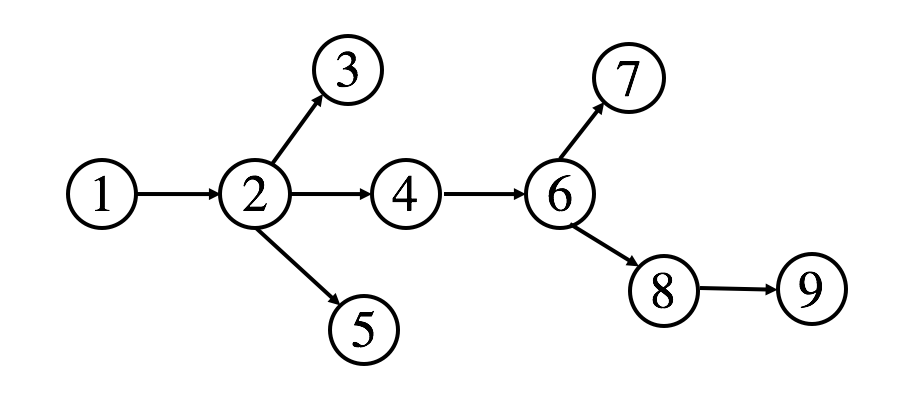
\includegraphics[width=0.32\textwidth,valign=c]{diffgraph} \\
			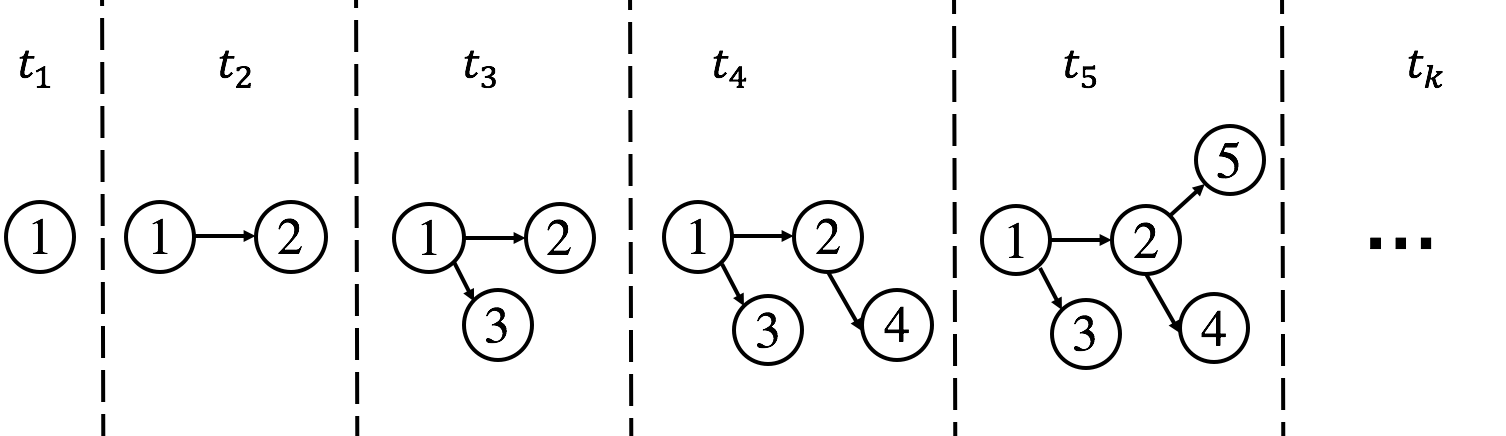
\includegraphics[width=0.51\textwidth,valign=c]{onediff}
		\end{tabular}
		\label{fig:example-diffusion-graph-construction}
	}
	\subfloat[] {
			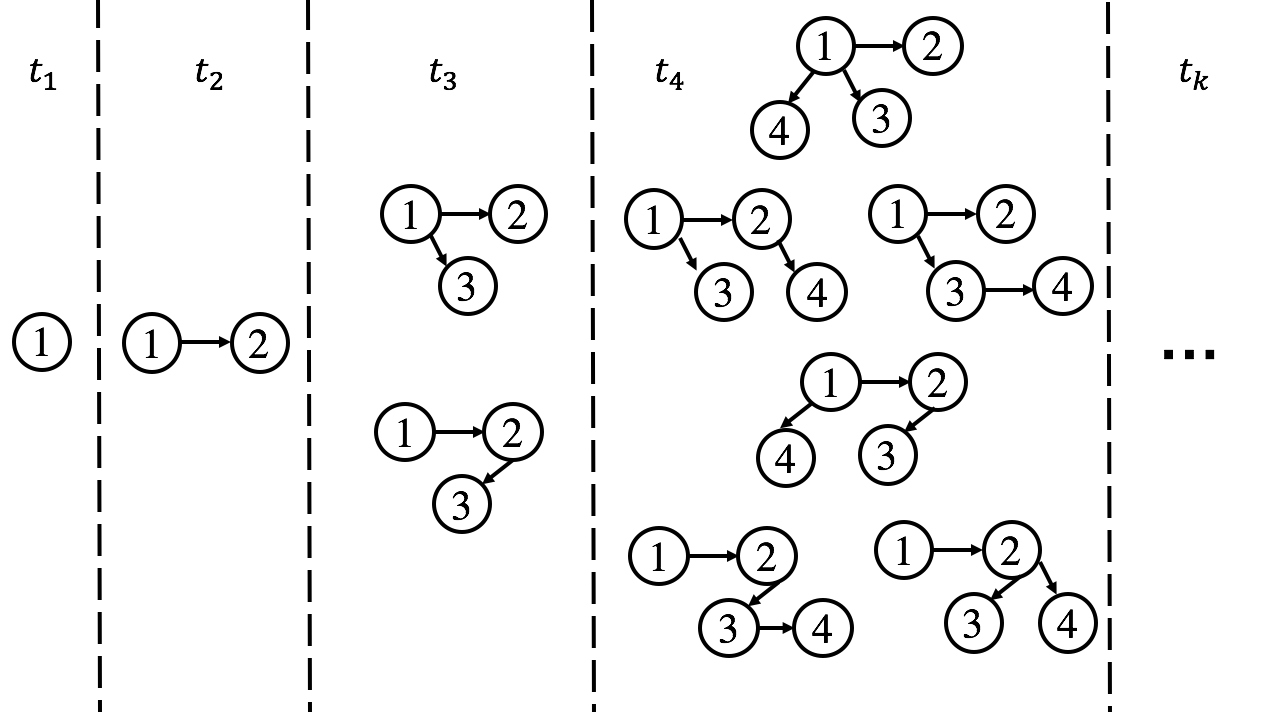
\includegraphics[height=0.2\textheight,valign=c]{diffusion}
			\vphantom{ % MAR: this is here to keep the label at the same position as for the other figures.
				\begin{tabular}{c}
					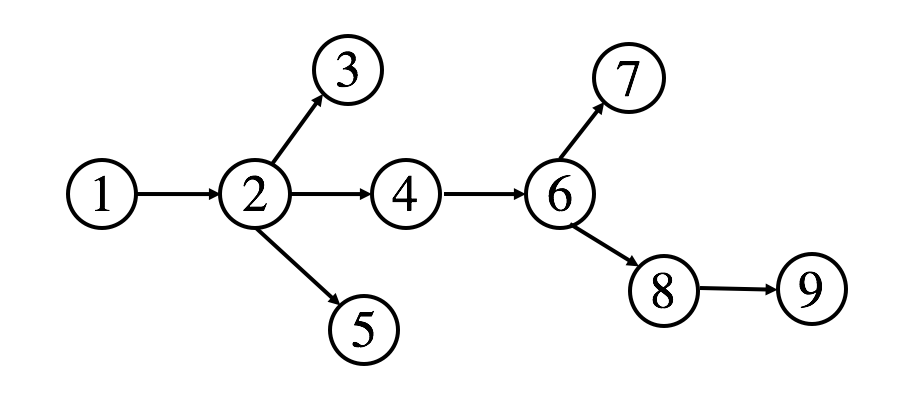
\includegraphics[width=0.32\textwidth,valign=c]{diffgraph} \\
					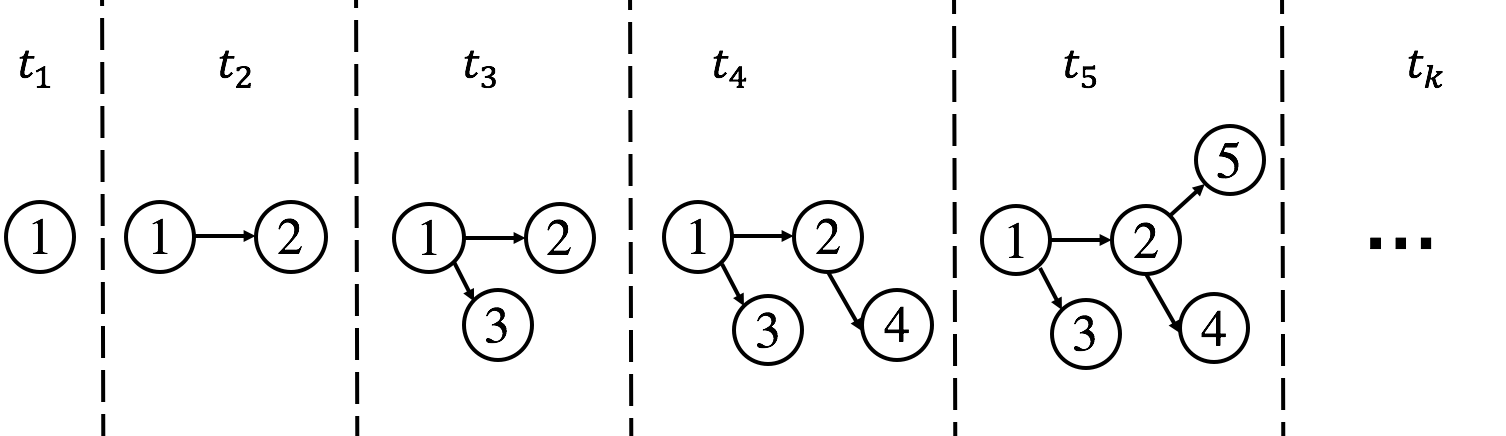
\includegraphics[width=0.51\textwidth,valign=c]{onediff}
				\end{tabular}
			}
			\label{fig:diffusion-scenarios} 
		}	
	
%	\begin{tabular}{cc}
%		\subfloat[] {
%			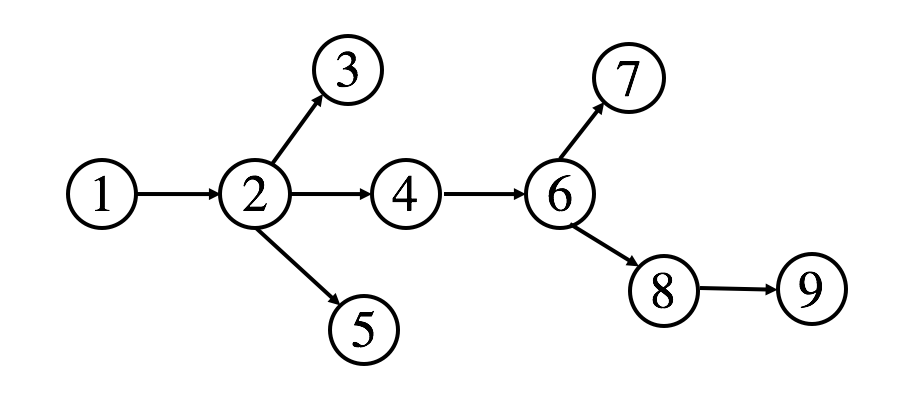
\includegraphics[width=0.32\textwidth,valign=c]{diffgraph}
%			\label{fig:example-diffusion-graph}
%	} &
%		\multirow{2}{*}[2em]{\subfloat[] {
%			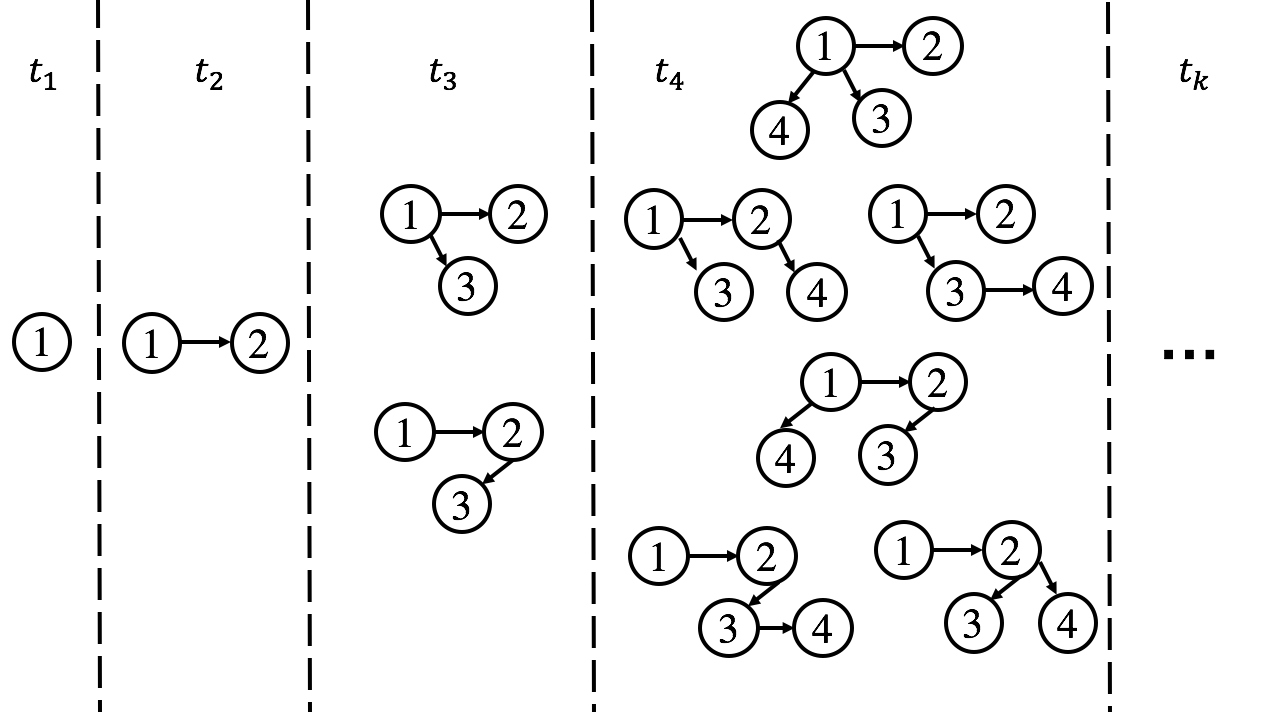
\includegraphics[height=0.2\textheight,valign=c]{diffusion}
%			\label{fig:diffusion-scenarios} 
%		}} \\
%	
%	%% new row	
%	\subfloat[] {
%		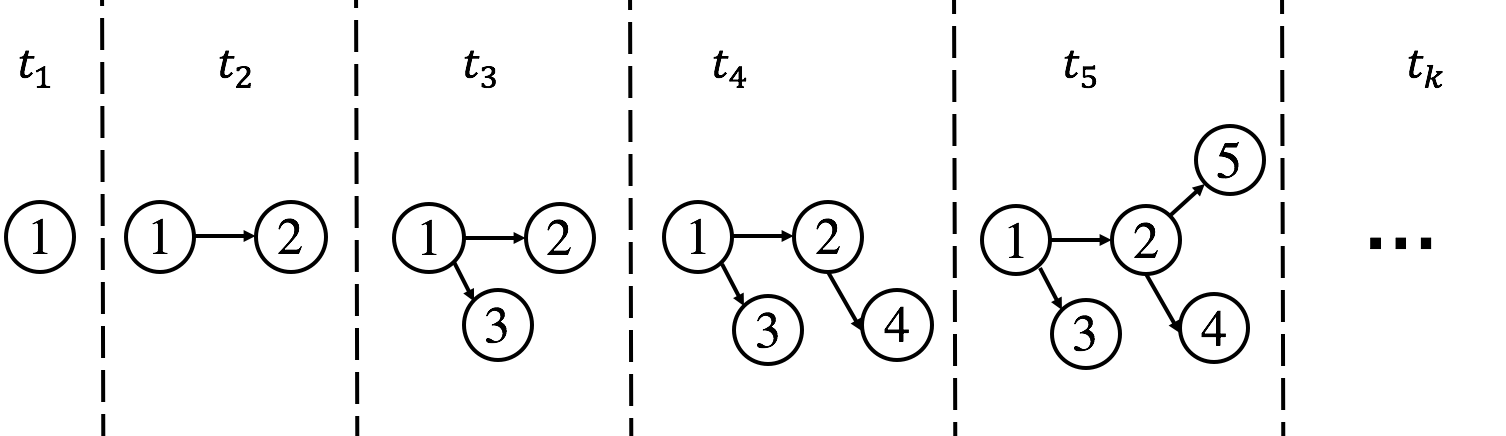
\includegraphics[width=0.51\textwidth,valign=c]{onediff}
%		\label{fig:diffusion-graph-construction}
%	} & \\
%	\end{tabular}



%	\subfloat[] {
%		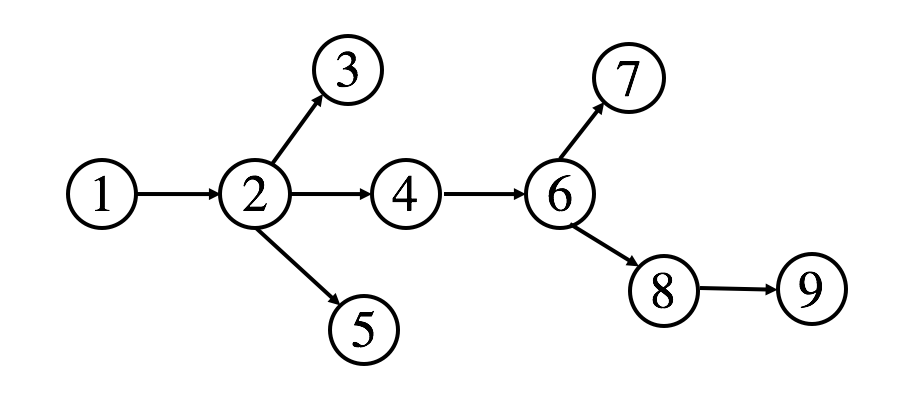
\includegraphics[width=\mywidth\textwidth,valign=c]{diffgraph}
%		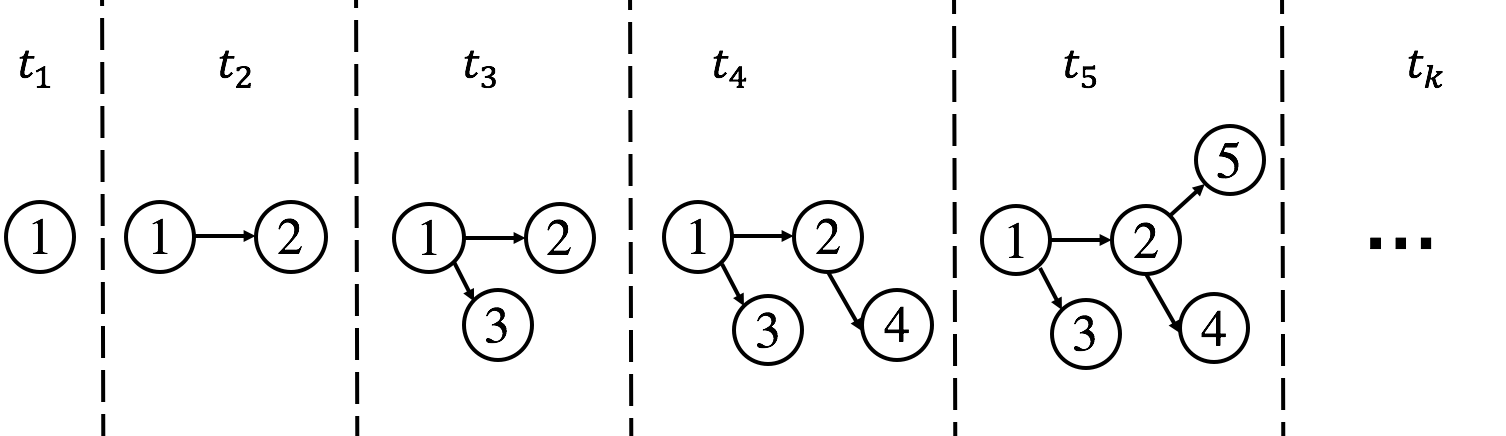
\includegraphics[width=\mywidth\textwidth,valign=c]{onediff}
%		\vphantom{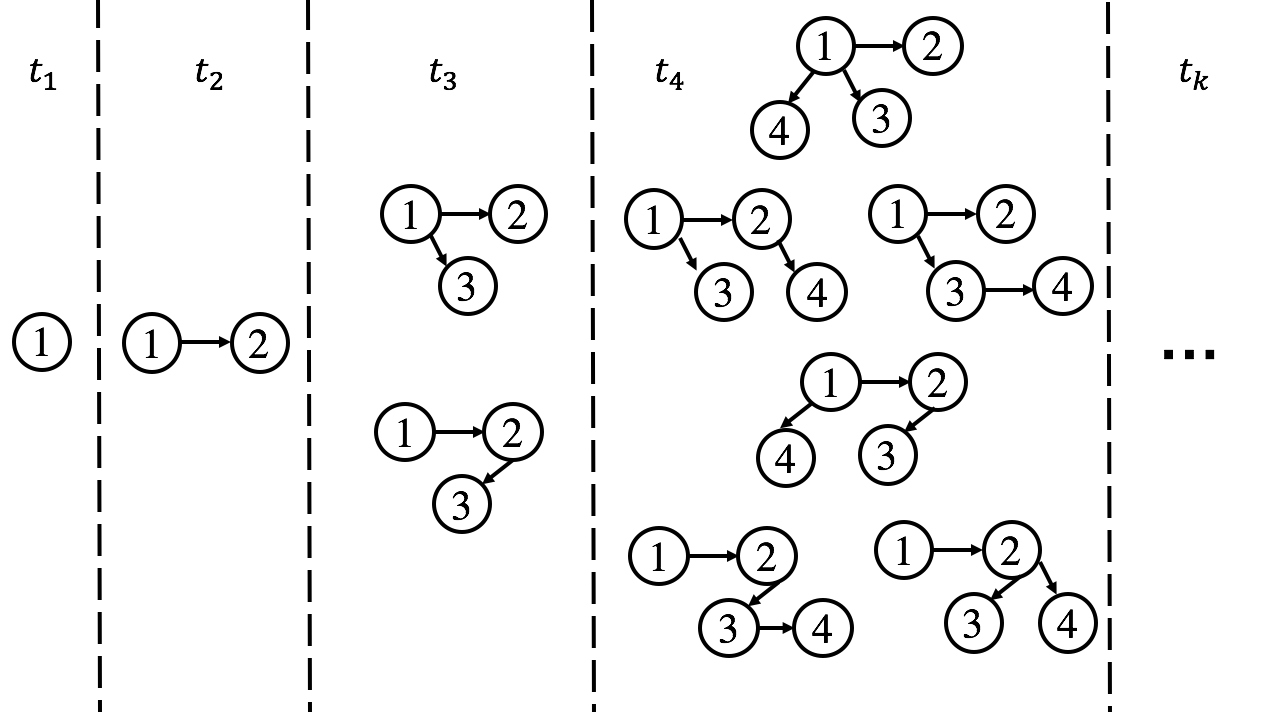
\includegraphics[height=\myheight\textheight,valign=c]{diffusion}}% MAR: this is here to keep the label at the same position as for the other figures.
%		\label{fig:side:a}
%	}
%	\hspace{0.2cm}
%	\subfloat[] {
%		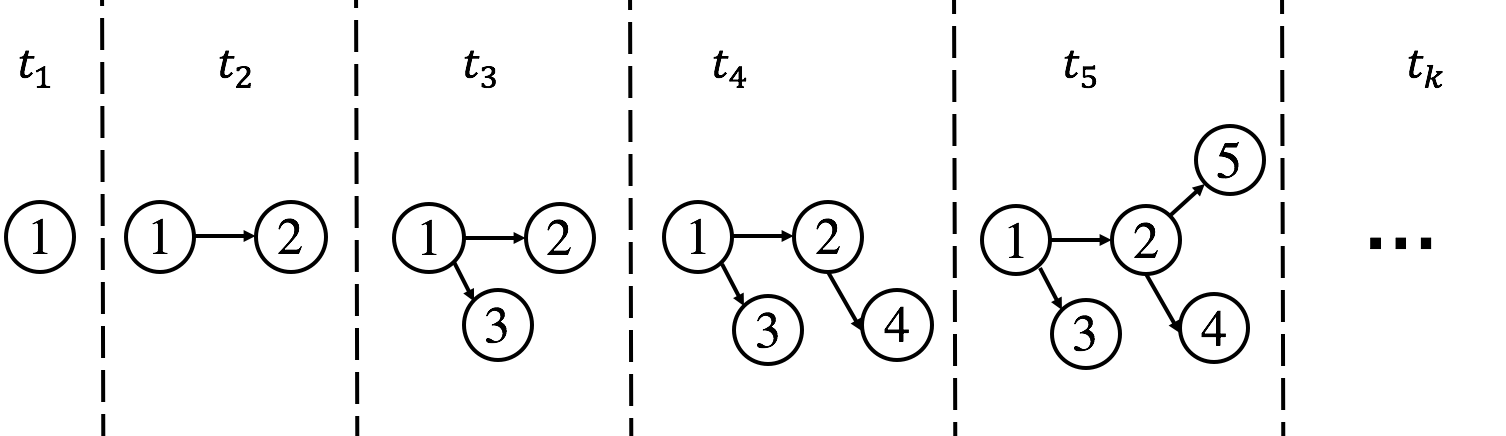
\includegraphics[width=\mywidth\textwidth,valign=c]{onediff}
%		\vphantom{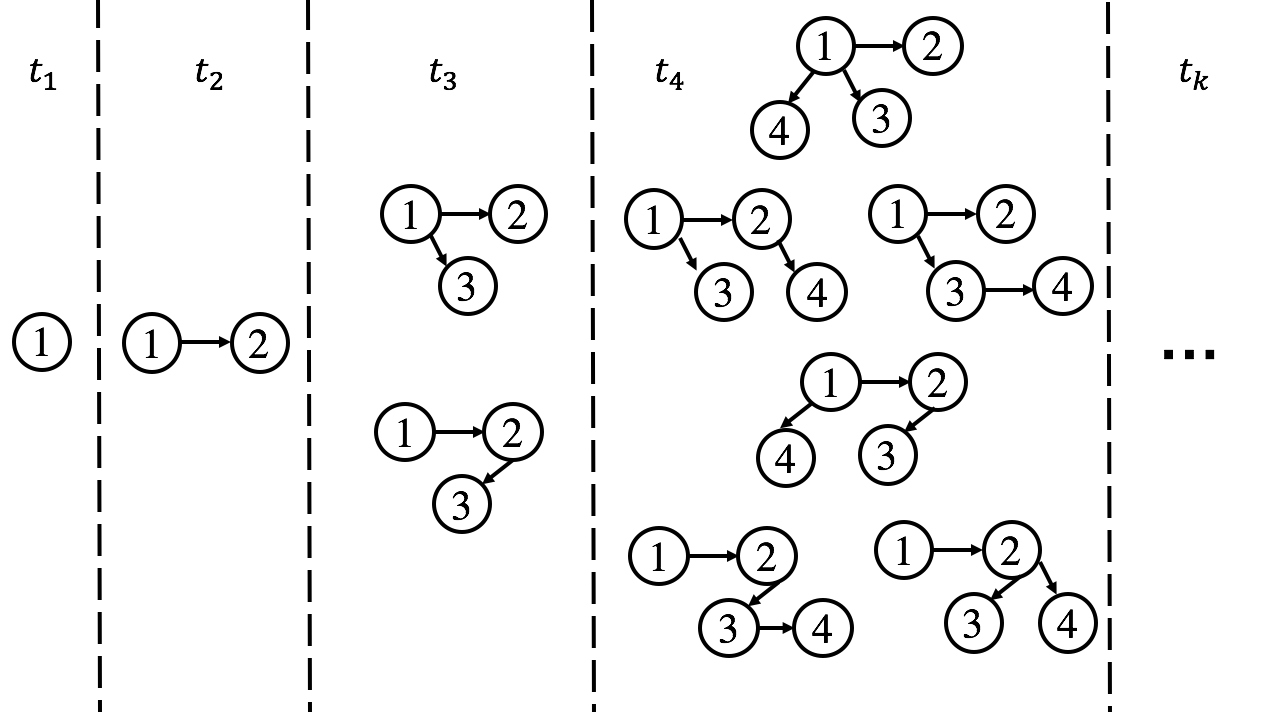
\includegraphics[height=\myheight\textheight,valign=c]{diffusion}}% MAR: this is here to keep the label at the same position as for the other figures.
%		\label{fig:side:b}
%	}
%	\hspace{0.2cm}
%	\subfloat[] {
%		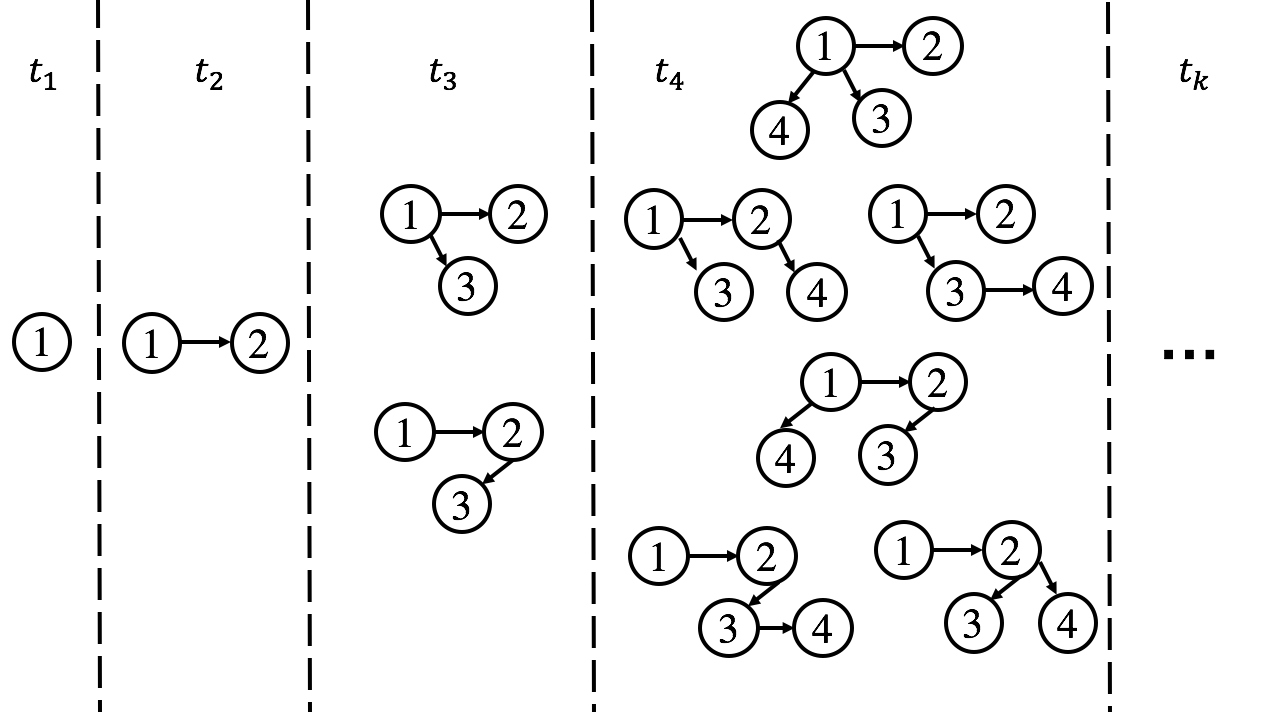
\includegraphics[height=\myheight\textheight,valign=c]{diffusion}
%		\label{fig:diffusion-scenarios}
%	}
	\caption{
		\textbf{(a)} An example of a diffusion tree \textbf{(top)} and its corresponding incremental diffusion process \textbf{(bottom)}.
		\textbf{(b)} Enumeration of all possible diffusion scenarios: 
		each retweet $v_k$ arrives at time $t_k$, and it can attach to any of the previous nodes, in any of the diffusion scenario constructed at time $t_{k-1}$.
		At time $t_k$ there are $(k-1)!$ diffusion scenarios, each with $k$ nodes.
	}
%	\captionmoveup
\end{figure*}

\textbf{Diffusion scenarios for retweet cascades.}
The diffusion tree is not observed for real Twitter retweet cascades, since the Twitter API does not expose the direct retweet relationships.
Instead, it assigns every retweet in the cascade to the original tweet.
%
%The underlying social graph is not observed for real Twitter retweet diffusions. 
%For data availability reasons, we only observe the order and timing of arrival of nodes.
%The Twitter API assigns every retweet to the original tweets, regardless of any retweeting chains.
%Consequently, 
Every retweet cascades constructed based on raw retweet information from the Twitter API resembles the graph in Fig.~\ref{fig:side:a}.
Due to this particular shape, we denote retweet cascades as \emph{stars}.
However, the API exposes the time of arrival of the retweets $t_i$.
We denote as a \emph{diffusion scenario} any valid diffusion tree that could be associated with the observed retweet star -- i.e., the edges in the diffusion tree respects the order of arrival of retweets.
Fig.~\ref{fig:side:b} shows four examples of diffusion scenarios associated with the star in Fig.~\ref{fig:side:a}.

\textbf{Constructing diffusion scenarios.}
%All possible diffusion scenarios need to be constructed. 
Fig.~\ref{fig:diffusion-scenarios} exemplifies a straight-forward method to enumerate all diffusion scenarios associated with the star in Fig.~\ref{fig:side:a}.
The node $v_1$ is the root node and it is published at time $t_1$;
tweet $v_2$ occurs at time $t_2$ and it is undoubtedly a direct retweet of $v_1$ -- a directed edge is drawn from $v_1$ to $v_2$. 
Tweet $v_3$ observed at $t_3$ can be a direct retweet of either tweet $v_1$ or tweet $v_2$.
Therefore, at time $t_3$ there are two possible diffusion scenarios: 
$G_1$ with the edge set $E = \lbrace (v_1, v_2), (v_1, v_3) \rbrace$ and $G_2$ with the edge set $E = \lbrace (v_1, v_2), (v_2, v_3) \rbrace$.
Similarly, $v_4$ can be a direct retweet of $v_1$, $v_2$ or $v_3$, in either $G_1$ or $G_2$.
Consequently, at time $t_4$ there are 6 possible diffusion scenarios.
The process continues until all nodes have been attached.
For an observed star of size $k$, there are $(k-1)!$ associated diffusion scenarios.
%Then two directed edges are drawn from $u_1$ to $u_3$ and $u_2$ to $u_3$. 
%Thus, two diffusion scenarios $G_1$ and $G_2$ are constructed due to the different users to retweet. 
%When the fourth user appears, it can retweet from $u_1$ to $u_3$ in any of previous diffusion scenarios. 
%This process will continue till the last user we observe. 
%Then All possible diffusion scenarios are built by sequentially adding users to previous diffusion scenarios.
%Eventually $(k-1)!$ number of diffusion scenarios are constructed when a cascade with the size of $k$ is observed.

\textbf{Probability of a diffusion scenario.}
%We denote as $v_i$ the user that has emitted the tweet $i$.
Given that in retweet cascades individual edges are not observed,
%Given that edges in diffusion scenarios are not observed,
%For diffusion scenarios, the edges (i.e. the direct retweet events) are not observed.
we define the probability of an edge $\mathds{P}\big((v_a, v_b)\big)$ as the likelihood that $u_b$ emitted tweet $v_b$ as a direct retweet of $v_a$.
%In line with previous work~\cite{crane2008robust,Mishra2016,Zhao2015,Shen2014,Yu2015},
We model two factors in the likelihood of retweeting:
firstly, users retweet \emph{fresh} content~\cite{Wu2007}.
The probability of the edge $(v_a, v_b)$ decays exponentially with the time difference $t_b - t_a$;
%The influence of user is exponential decay
secondly, users prefer to retweet locally influential users, also known as preferential attachment~\cite{Barabasi2005}.
We measure the local influence of a user using his number of followers~\cite{kwak2010twitter,Cha2010,Rizoiu2017}.
%The second assumption is that user prefers retweet from a user who has a lot of followers. 
%The number of followers a user has often related to its number of retweet. 
%More followers, a user has more channels he can get to broadcast his tweet to others, which increasing the likelihood of seeing by other users~\cite{1,2}.
%So the probability of retweeting can be express in the following equation:
We quantify the probability of an edge as:
\begin{equation} \label{eq:prob-edge}
	p_{ab} = \mathds{P}\big((v_a, v_b)\big) = \frac{m_a e^{-r({t_b-t_a})}}{\sum_{k=1}^{b-1} m_k e^{-r({t_b-t_k})}}
\end{equation}
%This equation describe the probability that user $u_b$ retweet from user $u_a$ 
where 
%$t_a$ and $t_b$ represent the retweet time of $u_a$ and $u_b$ respectively;
$m_a$ is the number of followers of the user of $u_a$ and
$r$ controls the temporal decay of the probability.
%$e^{-r({t_{b}-t_{a}})}$ express the probability decrease in exponential.
%$G$ is one diffusion scenario which user $u_b$ is added to.
%The probability of a diffusion scenario is intimately linked to the probability of an edge.

Under the assumption that retweeting events (i.e. edges) occur independently one from another, we obtain the probability of a diffusion scenario as:
%
%\textbf{Probability of diffusion scenarios.}
%As we describe above, one diffusion is constructed by a sequence of retweeting edges. 
%Each user $u_b$ will retweet from another user $u_a$ in its parent scenario with probability $\mathds{P}(u_a,u_b)$. 
%As each rewteet represent an egde $e$ in diffusion scenario.Thus, we can obtain the probability of a diffusion scenarios $\mathds{P}(G)$ via:
\begin{equation} \label{eq:prob-scenario}
	\mathds{P}(G) = \prod_{(v_a,v_b) \in E} \mathds{P}\big((v_a, v_b)\big)
\end{equation}

Note that the above assumption of independence of retweet events is a strong assumption.
Current state-of-the-art approaches~\cite{Mishra2016,Zhao2015} for modeling retweet cascades employ self-exciting point processes, in which the arrival of one event increases the probability of future events.
However, for our application of estimating the probability of a diffusion scenario it is the simplest assumption.
Additional arguments in its favor are also that we are studying networks of events
%\verify{RJA comment: Re. above assumption that retweeting events are independent of one another: it could be emphasised here that this assumption is valid because we are studying retweet cascades i.e. it is a network of events 
(in which each event is identified with unique user), not networks of users. 
The interdependence often observed in socially generated networks (like triadic closure)
%e.g. reciprocity, triangles by construction 
can be ignored in edge formation within a particular retweet cascade. 
%It's a directed acyclic graph (if I've got the right term?)}

%!TEX root = main.tex

\begin{figure*}[tbp]
	\newcommand\mywidth{0.19}
	\centering
	\subfloat[] {
		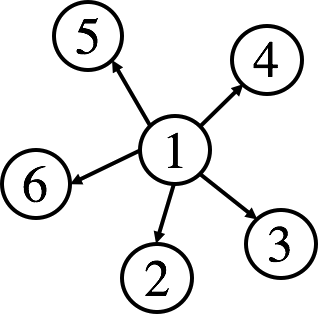
\includegraphics[width=0.14\textwidth,valign=c]{observcas}
		\vphantom{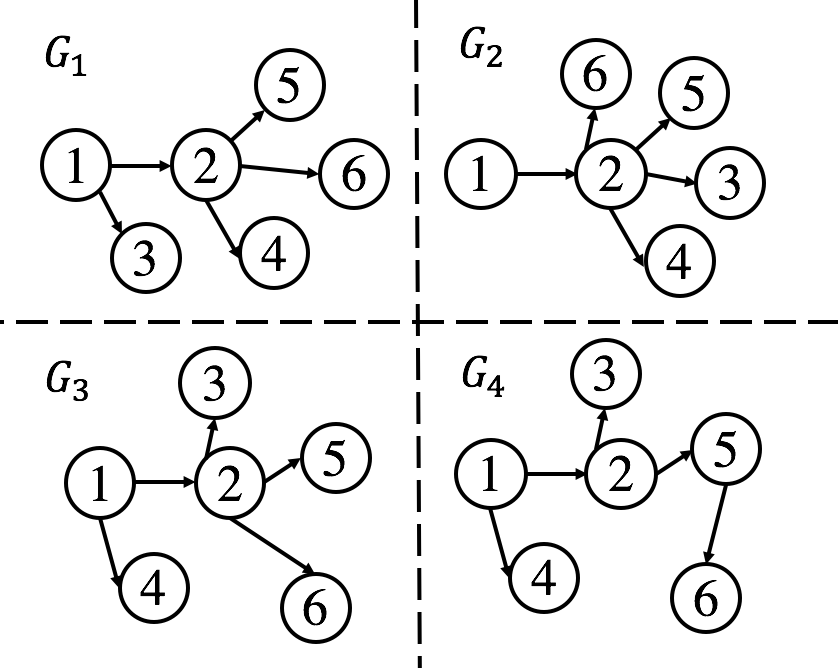
\includegraphics[height=\mywidth\textheight,valign=c]{somepossicas}}% MAR: this is here to keep the label at the same position as for the other figures.
		\label{fig:side:a}
	}
	\hspace{0.15cm}
	\subfloat[] {
		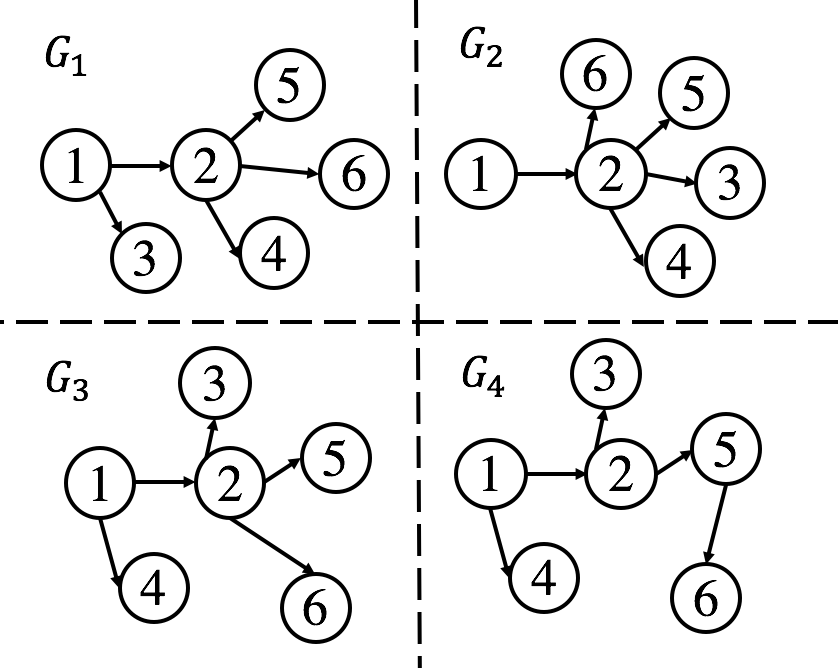
\includegraphics[height=\mywidth\textheight,valign=c]{somepossicas}
		\label{fig:side:b}
	}
	\hspace{0.15cm}
	\subfloat[] {
		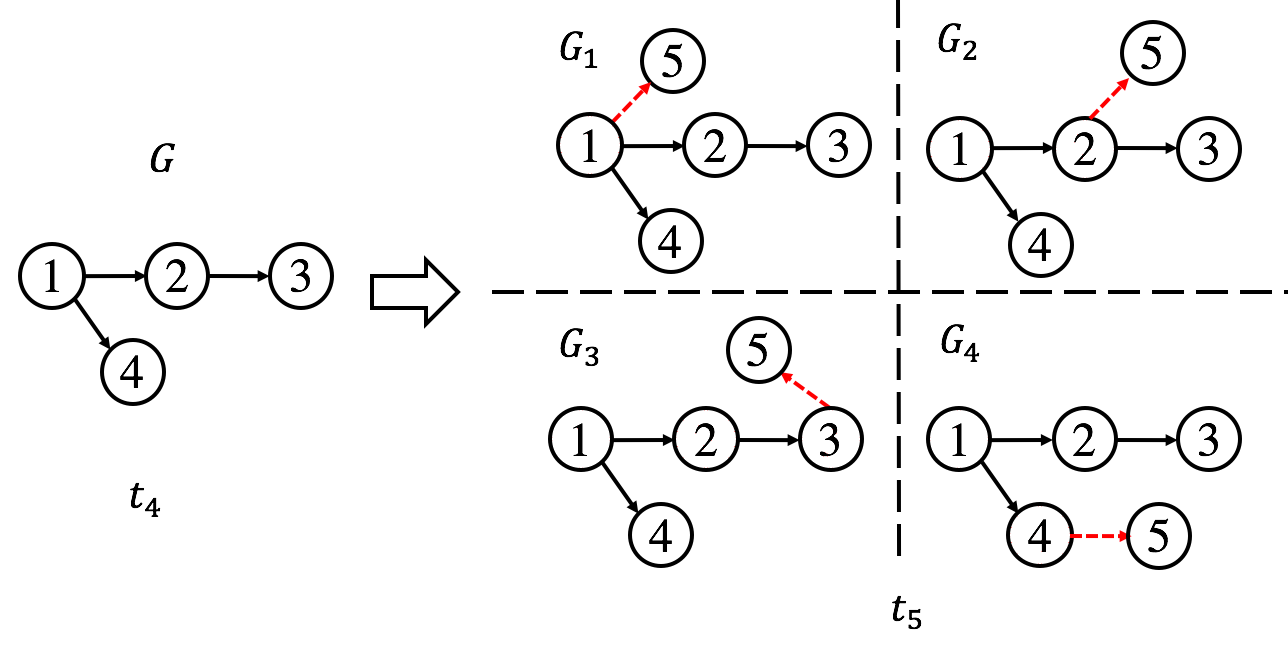
\includegraphics[height=\mywidth\textheight,valign=c]{gen_col}
		\label{fig:add-one-edge}
	}
	\caption{ 
		Modeling latent diffusions.
		\textbf{(a)} The schema of a retweet cascade as provided by the Twitter API, in which all retweets are attributed to the original tweet.
		\textbf{(b)} Four diffusion scenarios (out of 120 possible scenarios), associated with the retweet cascade in (a).
		\textbf{(c)} Intuition of the independent conditional model.
		A new node $v_5$ appears conditioned on one diffusion scenario $G$.
		Four new diffusion scenarios are generated as $v_5$ can attach to any of the existing nodes.
%		\hl{The influence of each of the nodes colored in red increases as $v_5$ attaches.}\verify{LX: unclear what ``increases'' refers to. suggest removing the red coloring and the sentence. i.e. this caption works equally well without the two highlighted sentences.}
	}
	\label{fig:holdout-ll}
%	\captionmoveup
\end{figure*}

\subsection{Computing tweet influence}
\label{subsec:user-influence}

\cite{Du2013} define user influence of a user $u$ as the average number of users in the social network who get in contact with the content emitted by $u$.
For retweet cascades the diffusion tree is not observed; it is impossible to directly measure user influence, apart from the root user.
We define the \emph{tweet influence} over a retweet cascade as the expected number of time it is retweeted -- direct retweets or descendants in a diffusion scenario --, over all possible diffusion scenarios associated with the given star.
Finally, we compute the influence of user $u$ as the sum of the influences of the tweets that $u$ authored.
We see that the definition in~\cite{Du2013} is a special case of our definition, in which the diffusion tree is observed.

\textbf{Tweet influence over one diffusion scenario.}
%Intuitively, given a diffusion scenarios G, the wider the spreading tweet, the more influential the user.
%We adopt the definition of influence as the number of average users that a target user can diffuse tweet to as in the previous work~\cite{3}.
%More precisely, let's say $U$ is the collection of users in G.
%
Let $z(v_i, v_k) \in G$ be a path in the diffusion scenario $G$ -- i.e a sequence of nodes which starts with $v_i$ and ends with $v_k$.
$\varphi(v_i | G)$ is the influence of $v_i$ given the diffusion scenario $G$ and it is computed as number of users reached from $v_i$ i.e. the number of descendants of $v_i$.
%, and $\varphi$ would be the  using a model of independent binomials to decide whether or not to take each hop in the path (instead of average number of reachable users … unclear what it means)
Formally:
%
%Consider a target user $v_i \in U$.
%This $v_i$ can diffuse its tweet to any user $v_k \in U $ though the path $z(v_i,v_k)$ which is from $v_i$ to $v_k$.
%The expected number of diffused user given a target user $v_i$ can be computed as: 
\begin{equation}
	\varphi(v_i|G) 	=  \sum_{v_k \in V(G)} \mathds{1} \big(z(v_i,v_k | G) ) \label{eq:infl-in-a-scenario}
\end{equation}
where $\mathds{1} \left( z(v_i,v_k|G) \right)$ is a function that takes the value 1 when the path from $v_i$ to $v_k$ exists in $G$.
%and the probability of path $z(v_i,v_k|G)$ can be obtained by the production over edges in this path $z$. That is:
%\begin{equation}
%	\mathds{P} \big\big(z(v_i,v_k|G) \big) = \prod_{\{u_a,u_b\} \in z} \mathds{P}\big(\{u_a,u_b\}\big).
%\end{equation}

\textbf{Tweet influence over a retweet cascade.}
We compute the influence of tweet $v_i$ over $VG$ -- all possible diffusion scenarios associated with a retweet cascade -- as:
%Since we do not have only one diffusion scenarios.
%We have multiple diffusion scenarios. 
%So the influence of target user  $\varphi(v_i)$ can be express as summing out $\varphi(v_i|G)$ over all possible diffusion scenarios:
\begin{align}
	\varphi(v_i) 	&= \sum_{G\in{VG}} \mathds{P}(G) \varphi(v_i|G) \nonumber \\
				&= \sum_{G\in{VG}} \mathds{P}(G) \sum_{v_k \in V(G)} \mathds{1}\big( z(v_i,v_k|G) \big) \label{eq:brute-user-infl}
\end{align}
%Where $VG$ is the collection of all possible diffusion scenarios that are generated from an observed retweet cascade. $G$ is one possible diffusion scenario in $VG$. The final user influence over all possible diffusion scenarios is:
%\begin{equation} \label{eq:user-infl-definition}
%\varphi(u) = \sum_{G\in{VG}}\mathds{P}\{G\} \sum_{u \in G}\prod_{\{u_a,u_b\} \in z}\frac{f(u_a)}{\sum_{u\in {G}}f(u)}e^{-r({t_{b}-t_{a}})}
%\end{equation}
It is intractable to directly evaluate Eq.~\eqref{eq:brute-user-infl}, plugged in with Eq.~\eqref{eq:prob-scenario} and~\eqref{eq:infl-in-a-scenario}, particularly due to the factorial number of diffusion scenarios in $VG$.
%It is challenging to compute Eq.~\eqref{eq:user-infl-definition} directly, particularly given that the number of diffusion scenarios is factorial with the size of diffusion cascade.
For example, there are $10^{156}$ diffusion scenarios for a cascade of 100 retweet.
We develop, in the next section, an efficient linear time algorithm to compute the influence of all tweets in a retweet cascade.
%To solve this problem, we develop an efficient algorithm in the next section.

\section{Efficient tweet influence computation}
\label{si-sec:efficient-algo}

The key observation is that each tweet $v_k$ is added simultaneously at time $t_k$ to all diffusion scenarios constructed at time $t_{k-1}$.
$v_k$ contributes only once to the tweet influence of each tweet that is found on the branch it attached to.
This process is exemplified in Fig.~\ref{fig:add-one-edge}.
Node $v_5$ is added to a given diffusion scenario, generating 4 new diffusion scenarios at time $t_5$.
We color in red the nodes whose influence increases as a result of adding node $v_5$.
%
%The key observation to efficiently compute user influence is that users $v_k$ are sequentially added to the diffusion scenarios constructed at time $t_k$. 
%If we ignore $v_k$, the structure of all previous diffusion scenarios remains unchanged. 
This allows to compute the tweet influence incrementally, by updating $\varphi(v_i), i < k$ at each time $t_k$.
We denote by $\varphi^k(v_i)$ the value of tweet influence of $v_i$ after adding node $v_k$.
As a result, we only keep track of how tweet influence increases over time steps and we do not require to construct all diffusion scenarios.

\subsection{Complete derivation of the recursive influence formula}

\textbf{Incremental construction of diffusion scenarios.}
Let $G^- \in VG^{k-1}$ be a diffusion scenario constructed at time $t_{k-1}$, with the set of nodes $V^- = \{ v_1,v_2,\cdots,v_{k-1} \}$.
When $v_k$ arrives, it can attach to any node in $V^-$, generating $k-1$ new diffusion scenarios $G_j^+$, with $V_j^+ = V^- \cup v_k$ and $E_j^+ = E^- \cup (v_j, v_k)$.
This process is exemplified in Fig.~\ref{fig:add-one-edge}.
We can write the set of scenarios at time $t_k$ as:
\begin{equation} \label{eq:diff-scenario-increase}
	VG^k = \left\lbrace G_j^+ = G^- \cup (v_j, v_k) \middle| \forall j < k, \forall G^- \in VG^{k-1} \right\rbrace
\end{equation}     
We write the tweet influence of $v_i$ at time $k$ as:
%
%
%Following the description in Sec.~\ref{sec:user-influence}, users are sequentially attached to previous diffusion scenarios. 
%When user $v_k$ is attached to previous diffusion scenarios constructed in time $k-1$ with a collection of users $U = \{u_1,u_2,u_3 \cdots,u_{k-1}\}$, for all $G \in VG^{k-1}$ at time $t_{k-1}$, each G can generates $k-1$ new scenario $G_i$ by adding edge $(v_i,v_k)$ where $G_i = G\cup (v_i,v_k)$.
%$G$ is the parent diffusion scenario of $G_i$.
% 
%So $\varphi^k(u_j)$ can be written as:
\begin{align}
	\varphi^k(v_i) &= \sum_{G^+ \in {VG^k}} \mathds{P}(G^+) \varphi(v_i|G^+) \nonumber \\
	^{cf.~\eqref{eq:diff-scenario-increase}} &= \sum_{G^- \in {VG^{k-1}}}\sum^{k-1}_{j=1}\mathds{P}(G_j^+) \varphi(v_i|G_j^+) \label{eq:infl-step-k}
\end{align}
Note that in Eq.~\eqref{eq:infl-step-k} we explicitly make use of how diffusion scenarios at time $k$ are constructed based on the diffusion scenarios at time $k-1$.

\textbf{Attach a new node $v_k$.}
We concentrate on the right-most factor in Eq.~\eqref{eq:infl-step-k} -- the tweet influence in scenario $G^+_j$.
We observe that the terms in Eq.~\eqref{eq:infl-in-a-scenario} can be divided into two:
the paths from $v_i$ to all other nodes except $v_k$ (i.e. the old nodes) and the path from $z(v_i, v_k)$.
We obtain:
%
%
%According to the definition of the user influence in one diffusion scenario, the influence of user $u_j$ in scenario $G_i$ at time $t_k$ can be written as:
%\begin{equation*}
%	\varphi(u_j|G_i)=\sum_{\substack{u_v \in {G_i}\\v>j}}\mathds{P}\{z(u_j,u_v|G_i)\}
%\end{equation*}
%$\sum_{u_v\in{G_i};v>j}\mathds{P}\{z(u_j,u_v|G_i)\}$ can be decomposed into two parts. The first part the probability of all the paths from $u_j$ to other users except $v_k$ and the second part is the probability of path from $u_j$ to $v_k$:
\begin{equation*}
	\varphi(v_i|G_j^+) = \sum_{\substack{v_l\in{G_j^+}\\l>i, l\neq k}} \mathds{1}\big(z(v_i,v_l|G_j^+)\big) + \mathds{1}\big(z(v_i,v_k|G_j^+)\big).
\end{equation*}
Note that a path that does not involve $v_k$ has the same probability in $G_j^+$ and in its parent scenario $G^-$:
\begin{equation*}
	\mathds{1}\big(z(v_i,v_l|G_j^+)\big) = \mathds{1}\big(z(v_i,v_l|G^-)\big), \text{ for } l > i, l \neq k
\end{equation*}
we obtain:
%We make use of the fact that $G_i$ without edge $(v_i,v_k)$ is equal to its parent scenario $G$. 
%So $\sum_{\substack{u_v\in{G_i}\\v>j\\v\neq k}}\mathds{P}\{z(u_j,u_v|G_i)\}$ is actually equal to $\sum_{\substack{u_v\in{G}\\v>j}}\mathds{P}\{z(u_j,u_v|G)\}$ then:
\begin{align}
				\varphi(v_i|G_j^+) 		&= \sum_{\substack{v_l\in{G^-}\\l>i}} \mathds{1}\big(z(v_i,v_l|G^-)\big) + \mathds{1}\big(z(v_i,v_k|G_j^+)\big) \nonumber \\
^{cf.~\eqref{eq:infl-in-a-scenario}}	&= \varphi(v_i | G^-) + \mathds{1}\big(z(v_i,v_k|G_j^+)\big) \label{eq:infl-step-k+1}
\end{align}
Combining Eq.~\eqref{eq:infl-step-k} and~\eqref{eq:infl-step-k+1}, we obtain:
\begin{align}
\varphi^k(v_i) &= \sum_{\substack{G^-\\\in VG^{k-1}}}\sum^{k-1}_{j=1} \mathds{P}(G_j^+) \bigg[ \varphi(v_i | G^-) + \mathds{1}\big(z(v_i,v_k|G_j^+)\big) \bigg] \nonumber \\
        &= \underbrace{\sum_{G^- \in {VG^{k-1}}} \varphi(v_i | G^-) \sum^{k-1}_{j=1}\mathds{P}(G_j^+) }_{A} \nonumber \\
        &+ \underbrace{\sum_{G^- \in {VG^{k-1}}}\sum^{k-1}_{j=1} \mathds{P}(G_j^+) \mathds{1}\big(z(v_i,v_k|G_j^+)\big) }_{m_{ik}}. \label{eq:two-parts}
\end{align}

\textbf{Tweet influence at previous time step $t_{k-1}$.}
Given the definition of $G_j^+$ in Eq.~\eqref{eq:diff-scenario-increase}, we obtain that $\mathds{P}(G_j^+) = \mathds{P}(G^-)\mathds{P}\big((v_j,v_k)\big)$.
Consequently, part $A$ in Eq.~\eqref{eq:two-parts} can be written as:
\begin{align}
	A 	&= \sum_{G^- \in {VG^{k-1}}} \varphi(v_i | G^-) \sum^{k-1}_{j=1} \mathds{P}(G^-)\mathds{P}\big((v_j,v_k)\big) \nonumber \\
		&= \sum_{G^- \in {VG^{k-1}}} \varphi(v_i | G^-) \mathds{P}(G^-) \sum^{k-1}_{j=1} \mathds{P}\big((v_j,v_k)\big) \nonumber \\
		&= \sum_{G^- \in {VG^{k-1}}} \mathds{P}(G^-) \varphi(v_i | G^-)  \nonumber \\
	^{cf.~\eqref{eq:brute-user-infl}}	&= \varphi^{k-1}(v_i) \label{eq:past-infl}
\end{align}
Consequently, $A$ is the tweet influence of $v_i$ at the previous time step $t_{k-1}$.
Note that $\sum^{k-1}_{j=1} \mathds{P}\big((v_j,v_k)\big) = 1$ because $v_k$ is necessarily the direct retweet of one of the previous nodes $v_j, j < k$ of the retweet cascade.
%For part $A$, what we interested in is that how A relate to $\varphi(u_j)$ in previous timestamps $t_{k-1}$. 
%We use the fact again that $G_i = G \cup (v_i,v_k)$. 
%Thus $\mathds{P}\{G_i\} = \mathds{P}\{G\}\mathds{P}(v_i,v_k)$. Then A can be expressed as:
%\[
%\begin{alignedat}{3}
%A &= \sum_{G\in{VG^{k-1}}}\sum^{k-1}_{i=0}\mathds{P}\{G\}\mathds{P}(v_i,v_k)\sum_{\substack{u_v\in{G}\\v>j}}\mathds{P}\{z(u_j,u_v|G)\}\\
%  &= \sum_{G\in{VG^{k-1}}}\mathds{P}\{G\}\sum^{k-1}_{i=1}\mathds{P}(v_i,v_k)\sum_{\substack{u_v\in{G}\\v>j}}\mathds{P}\{z(u_j,u_v|G)\}\\
%\end{alignedat}
%\]
%The next importance fact is that $\mathds{P}(v_i,v_k)$ describe the probability that $v_k$ retweet from any previous user $v_i$ where $v_i \in \{u_1,u_2 ,\cdots, u_{k-1}\} $. Thus $\sum^{k-1}_{i=1}\mathds{P}(v_i,v_k) $ need to normalize to 1.
%
%\[
%\begin{alignedat}{3}
%A &= \sum_{G\in{VG^{k-1}}}\mathds{P}\{G\}\sum_{\substack{u_v\in{G}\\v>j}}\mathds{P}\{z(u_j,u_v|G)\}\\
% &= \sum_{G\in{VG^{k-1}}}\mathds{P}\{G\}\varphi(u_j|G)\\
%\end{alignedat}
%\]
%Finally, A fits in the definition of user influence over all diffusion scenarios at $t_{k-1} $, that is:
%\[
%A  =\varphi^{k-1}(u_j)
%\]

%!TEX root = main.tex

\begin{figure*}[tbp]
	\centering
	\begin{minipage}{\textwidth}
		 \[
 \underbrace{\left[
\begin{matrix}
 \textcolor{gray}{1}  &\textcolor{blue}{m_{12}}  &\textcolor{red}{m_{13}}   &\textcolor{ForestGreen}{m_{14}}      & \cdots    & m_{1n} \\
 0                    &\textcolor{blue}{1}   	 &\textcolor{red}{m_{23}}   &\textcolor{ForestGreen}{m_{24}}      & \cdots    & m_{2n} \\
 0                    &0             			 &\textcolor{red}{1}   	    &\textcolor{ForestGreen}{m_{34}}      & \cdots    & m_{3n} \\
 0                    &0             			 &0             			&\textcolor{ForestGreen}{1}   		& \cdots    & m_{4n} \\
 \vdots    		      &\vdots            		 & \vdots       			&\vdots       				    & \ddots    & \vdots \\
 0         		      &0             			 &0                         &0             				    & \cdots    & 1      \\
\end{matrix}   
\right]}_{\textbf{M}} 
 \underbrace{\left[
\begin{matrix}
 1         &\textcolor{gray}{p_{12}}       &\textcolor{blue}{p_{13}}       &\textcolor{red}{p_{14}}        & \cdots    & p_{1n} \\
 0         &1             	    		   &\textcolor{blue}{p_{23}}       &\textcolor{red}{p_{24}}        & \cdots    & p_{2n} \\
 0         &0             				   &1					   		   &\textcolor{red}{p_{34}}         & \cdots    & p_{3n} \\
 0         &0             				   &0             				   &1					  		    & \cdots    & p_{4n} \\
 \vdots    &\vdots            			   & \vdots       				   & \vdots       				    & \ddots    & \vdots \\
 0         &0             				   &0                              &0             					& \cdots    & 1      \\
\end{matrix}   
\right]}_{\textbf{P}}
\]
\[
\begin{alignedat}{3}
&\begin{array}{rl}&m_{11} = 1 \end{array} &k =1\ \ \ \ \ &\\ 
&\begin{array}{rl}&m_{12} =p_{12}m_{11}\end{array} &k= 2 \ \ \ \ &\left[\textcolor{gray}{p_{12}}\right]\left[\textcolor{gray}{m_{11}}\right] = 
\left[\textcolor{blue}{m_{12}}\right]\\
&\begin{array}{rl}
	&m_{13} =p_{13}m_{11}+ p_{23}m_{12}\\
	&m_{23} =p_{13}m_{21}+ p_{23}m_{22}
\end{array}
\Bigg\} &k = 3 \ \ \ \ 
&\left[
\begin{matrix}
\textcolor{gray}{1}  &\textcolor{blue}{m_{12}} \\
0                    &\textcolor{blue}{1}   	
\end{matrix}
\right]
\left[
\begin{matrix}
\textcolor{blue}{p_{13}}\\
\textcolor{blue}{p_{23}}
\end{matrix}
\right]=
\left[
\begin{matrix}
\textcolor{red}{m_{13}}\\
\textcolor{red}{m_{23}}
\end{matrix}
\right]\\
&\begin{array}{rl}
	&m_{14} =p_{14}m_{11}+ p_{24}m_{12}+ p_{34}m_{13}\\
	&m_{24} =p_{14}m_{21}+ p_{24}m_{22}+ p_{34}m_{23}\\
    &m_{34} =p_{14}m_{31}+ p_{24}m_{32}+ p_{34}m_{33}
\end{array}
\Bigg\} &k = 4 \ \ \ \ 
&\left[
\begin{matrix}
 \textcolor{gray}{1}  &\textcolor{blue}{m_{12}}  &\textcolor{red}{m_{13}}\\
 0                    &\textcolor{blue}{1}   	 &\textcolor{red}{m_{23}}\\
 0                    &0             			 &\textcolor{red}{1}   	 
\end{matrix}
\right]
\left[
\begin{matrix}
\textcolor{red}{p_{14}}\\
\textcolor{red}{p_{24}}\\
\textcolor{red}{p_{34}}
\end{matrix}
\right]=
\left[
\begin{matrix}
\textcolor{ForestGreen}{m_{14}}\\
\textcolor{ForestGreen}{m_{24}}\\
\textcolor{ForestGreen}{m_{34}}
\end{matrix}
\right]\\
\end{alignedat}
\]
	\end{minipage}
	\caption{
		Exemplification of the efficient computation of the first four columns of matrix $M$.
%		Algorithm~\ref{alg:casin} which describes in the previous section can also be written in  matrix processing, The element of the matrix $m_{ij}$ can be obtained by the following steps:	
%		According to the equation(7), 
		Each $k^{th}$ column vector of matrix $M$ is colored correspondingly with the column vector in $P$ used in the multiplication.
%		
%		
%		can be computed by sub-matrix with size of $k-1\times k-1$ in $m_{ji}$ multiplying $k$th column vector with same color in $p_{ji}$.
%		Therefore, given matrix $p_{ji}$, from $k = 1$, $M$ can be computed incrementally follow the process above.		
	}
	\label{fig:matrix-operations-example}
\end{figure*}

\textbf{Contribution of $v_k$.}
With $A$ being the influence of $v_i$ at the previous time step, intuitively $m_{ik}$ is the contribution of $v_k$ to the influence of $v_i$.
Knowing that:
\begin{align*}
	\mathds{P}(G_j^+) &= \mathds{P}(G^-)\mathds{P}\big((v_j,v_k)\big) \text{ and } \\
	\mathds{1}\big(z(v_i,v_k|G_j^+)\big) &= \mathds{1}\big(z(v_i,v_j|G^+_j)\big) \mathds{1}\big((v_j,v_k)\big) \\
	 &= \mathds{1}\big(z(v_i,v_j|G^-)\big)
\end{align*}
we write $m_{ik}$ as:
%
%The only problem left is to compute $M_{jk}$ which is part $B$. The basic idea here is also to derive the relation between $t_k$ and $t_k-1$ by using the observation we have discussed.  
%\begin{align}
%B = M_{jk} &= \sum_{G\in{VG^{k-1}}}\sum^{k-1}_{i=1}\mathds{P}(G_i)\mathds{P}\{z(u_j,v_k|G_i)\} \nonumber \\
%		   &= \sum_{G\in{VG^k}}\mathds{P}\{G\}\mathds{P}\{z(u_j,v_k|G)\}       
%\end{align}
%We know that $G_i = G\cup (v_i,v_k)$ thus $\mathds{P}\{G_i\} = \mathds{P}\{G_i\} \mathds{P}(v_i,v_k)$ and $\mathds{P}\{z(u_j,v_k|G_i)\} = \mathds{P}\{z(u_j,v_i|G)\}\mathds{P}(v_i,v_k)$ so: 
\begin{align}
	m_{ik} &= \sum_{G^- \in {VG^{k-1}}} \sum^{k-1}_{j=1} \mathds{P}(G^-)\mathds{P}\big((v_j,v_k)\big) \mathds{1}\big(z(v_i,v_j|G^-)\big) \nonumber \\
           &= \sum^{k-1}_{j=1} \mathds{P}\big((v_j,v_k)\big) \underbrace{ \sum_{G^- \in {VG^{k-1}}} \mathds{P}(G^-) \mathds{1}\big(z(v_i,v_j|G^-)\big)}_{M_{ij}} \nonumber \\  
		   &= \sum^{k-1}_{j=1} \mathds{P}\big((v_j,v_k)\big) M_{ij} \label{eq:M-ik}
\end{align}
%By comparing the final and the original form of B:
%\[
%\begin{alignedat}{3}
%B 			   &= \sum_{G\in{VG^k}}\mathds{P}(G)\mathds{P}\{z(u_j,v_k|G)\}\\
%               &= \sum^{k-1}_{i=1}\bigg[\mathds{P}^2(v_i,v_k)\sum_{G\in{VG^{k-1}}}\mathds{P}(G)\mathds{P}\{z(u_j,v_i|G)\}\bigg]\\ 
%M_{jk} &= \sum_{i=1}^{k-1}\bigg[\mathds{P}^2(v_i,v_k)M_{ji}\bigg]
%\end{alignedat}
%\]
An alternative interpretation for $m_{ik}$ is the influence of $v_i$ over $v_k$.
Eq.~\eqref{eq:M-ik} can be intuitively understood as the expected influence of $v_i$ over a newly attached node $v_k$ is proportional to the influence of $v_i$ over each already attached node $v_j$ multiplied with the likelihood that $v_k$ attached itself to $v_j$.
We obtain the formula of the the expected influence of a node $v_i$ over another node $v_k$ as:
%
%Through this equation we can observed that $M_{jk}$ which is the influence $u_j$ over $v_k$ can be recursively calculated using $\mathds{P}(v_i,v_k)$ and $M_{ji}$ which is influence $u_j$ over $v_i$ where $v_i$ is the user that $v_k$ attach to.  Any user in a diffusion can not have the influence on any previous user because there is no directed path pointing back to the previous user. Therefore $M_{jk}(j>k)$ equals zero and the influence on the user itself set to one in default.
\begin{equation} \label{eq:Mij}
m_{ik}=
\left\{
\begin{array}{ll}
	\sum^{k-1}_{j=1}m_{ij}\mathds{P}\big((v_j, v_k)\big) &,i < k \\
	1 & ,i = k \\
	0 & ,i > k.
\end{array}
\right.
\end{equation} 
%where $P_{ik}$ is $\mathds{P}^2(v_i,v_k)$.

\textbf{Recursive computation of tweet influence.}
Using Eq~\eqref{eq:two-parts} and~\eqref{eq:past-infl}, we can recursively compute the influence of $v_i$ at time $t_k$ as:
%For part B, based on the description in Sec~\ref{sec:user-influence}, we observe that the only difference between diffusion scenarios in $t_k$ and $t_{k-1}$ is where $v_k$ place, which indicates the change of influence for each previous user from $t_{k-1}$ to $t_k$ solely relay on $v_k$. 
%So far, we already separate A which is user influence $\varphi^{k-1}(u_j)$ in $t_{k-1}$ from user influence $\varphi^{k}(u_j)$in $t_k$. 
%Therefore, the rest of the part B is actually the influence that user $v_k$ contribute when it is added at $t_k$. 
%If we define $M_{jk} = B = \sum_{G\in{VG^{k}}}\mathds{P}(G)\mathds{P}\{z(u_j,v_k|G)\}$ as $M_{jk}$ which is the influence that $u_j$ exerts on $v_k$.
\begin{align}
	\varphi^k(v_i) &= \varphi^{k-1}(v_i) + m_{ik} \nonumber \\
				   &= \varphi^{k-2}(v_i) + m_{i(k-1)} + m_{ik} \nonumber \\
				   &= \sum_{j=1}^k m_{ij}. 
\end{align}
with $m_{ij}$ as defined in Eq.~\eqref{eq:Mij}.
Intuitively, the influence of $v_i$ at time $t_k$ is the sum of the expected influence over each of the nodes in the diffusion scenario.

%Therefore, the influence of $u_j$ computed at time $t_k$ when $v_k$ is added can be obtained through the influence of $u_j$ at $t_{k-1}$ and the influence that $v_k$ contribute to $u_j$. 
%Then the $\varphi^k(u_j)$ can be calculated by summing out the influence that $u_j$ has over subsequently arrived users $(u_{j+1}, \ldots , v_k)$
%\begin{equation}
%\varphi^k(u_j) = \sum_{i=1}^k M_{ji} \text{   , with } M_{ji} = 0, \text{   for } i \leq j
%\end{equation}

\subsection{Tweet influence algorithm}

We define two matrices:
matrix $P = [ P_{ij} ]$, with $P_{ij} = \mathds{P}\big((v_i, v_j)\big)$.
Element $P_{ij}$ of the matrix $P$ is the probability that tweet $v_j$ is a direct retweet of tweet $v_i$;
matrix $M = [ m_{ij} ]$, with $m_{ij}$ defined in Eq.~\eqref{eq:Mij}.
Element $m_{ij}$ of matrix $M$ is the contribution of $v_j$ to the influence of $v_i$.
Alternatively, $m_{ij}$ can be interpreted as the influence of $v_i$ on $v_j$.

From Eq.~\eqref{eq:Mij} follows the formula for computing iteratively the columns of matrix $M$:
\begin{equation} \label{eq:Mij-matrix}
M_{ \cdot j}=
\left[
\begin{array}{c}
M_{[1..j-1, 1..j-1]} \times P_{[1:j-1,j]} \\
1 \\
0 \\
0 \\
\vdots \\
0 
\end{array}
\right]
\end{equation}
with the value 1 occurring on line $j$.
For each column $j$, we compute the first $j-1$ elements by multiplying the sub-matrix $M_{[1..j-1, 1..j-1]}$ with the first $j-1$ elements on the $j^{th}$ column of matrix $P$.
The computation of matrix $M$ finishes in linear time, after $n$ steps, where $n$ is the total number of retweets in the retweet cascade.
Fig.~\ref{fig:matrix-operations-example} demonstrated the computation of the first four columns in $M$.
%Algorithm~\ref{alg:casin} gives an overview of the efficient influence computation algorithm.
